\documentclass[journal,12pt,twocolumn]{beamer}
\usetheme{CambridgeUS}
\usepackage[utf8]{inputenc}

\usepackage{tfrupee}
\usepackage{enumitem}
\usepackage{amsmath}
\usepackage{amssymb}
\usepackage{graphicx}

\providecommand{\sbrak}[1]{\ensuremath{{}\left[#1\right]}}
\providecommand{\lsbrak}[1]{\ensuremath{{}\left[#1\right.}}
\providecommand{\rsbrak}[1]{\ensuremath{{}\left.#1\right]}}
\providecommand{\brak}[1]{\ensuremath{\left(#1\right)}}
\providecommand{\lbrak}[1]{\ensuremath{\left(#1\right.}}
\providecommand{\rbrak}[1]{\ensuremath{\left.#1\right)}}
\providecommand{\cbrak}[1]{\ensuremath{\left\{#1\right\}}}
\providecommand{\lcbrak}[1]{\ensuremath{\left\{#1\right.}}
\providecommand{\rcbrak}[1]{\ensuremath{\left.#1\right\}}}



\newcommand{\myvec}[1]{\ensuremath{\begin{pmatrix}#1\end{pmatrix}}}
\let\vec\mathbf

\title{Assignment 8}
\author{Ravula Karthik (AI21BTECH11024)}
\date {June 2022}
\begin{document}
	\begin{frame}
		\titlepage 
	\end{frame}
	
	\begin{frame}{Question : EX 6.41}
		
	The random variable $x$ is of discrete type taking the values $ x_n $ with $P\cbrak{x=x_1} = p_n$ and the
	random variable y is of continuous type and independent of $x$. Show that if $z = x + y$ and
	$w = xy$, then
	\end{frame}
	\begin{frame}{Solution}
		
	
	(a)
	
	\begin{figure}[H]
		\centering
		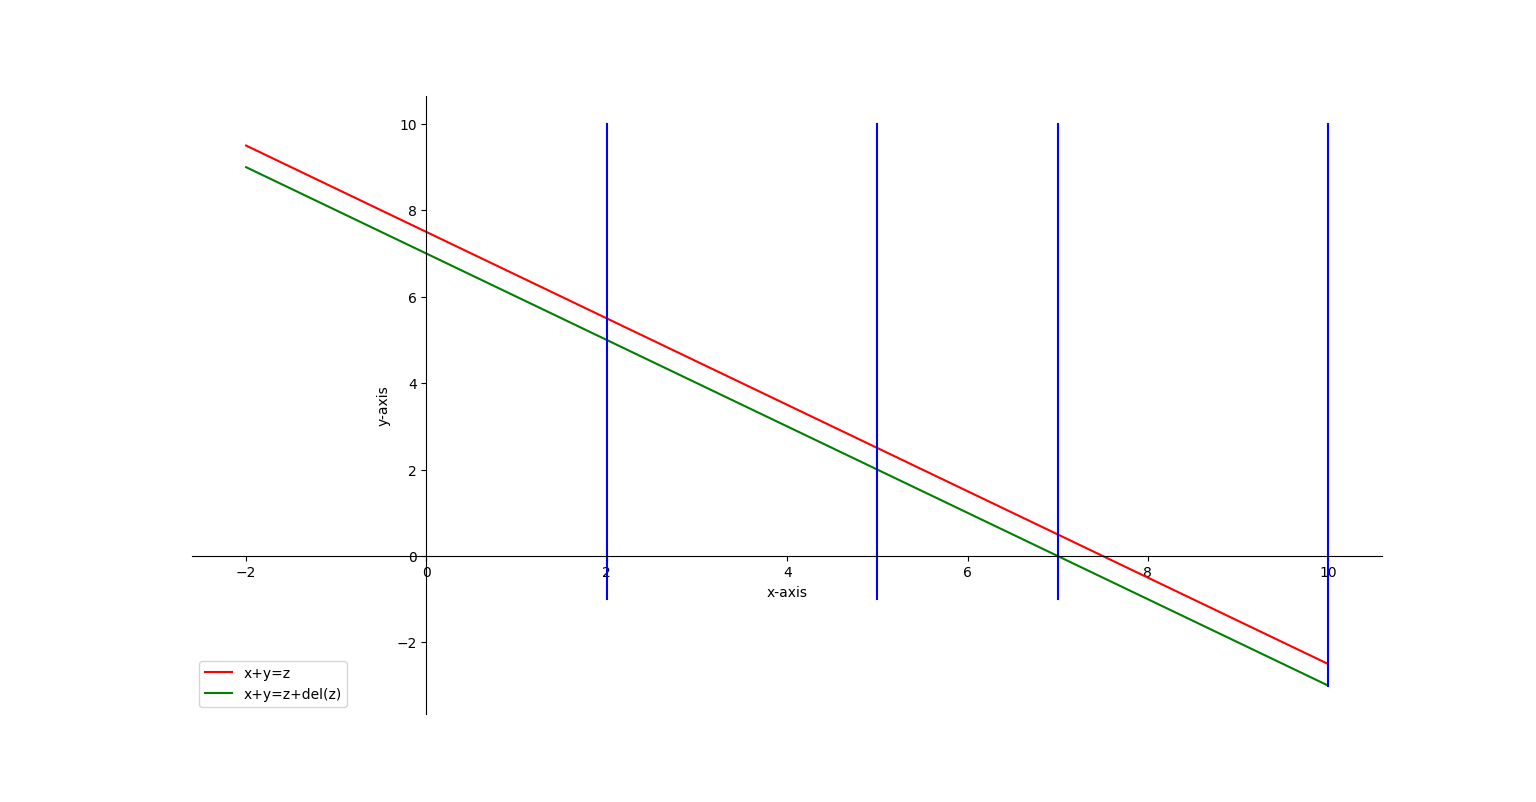
\includegraphics[width=\columnwidth]{figs/assign_8_Figure_1.png}
		\label{Fig1}	
	\end{figure}

	\end{frame}
	
	\begin{frame}
		\underline{Line masses}
		
		\begin{align}
			P\cbrak{x=x_n ,z-x_n \le \underline{y} \leq z-x_n +\Delta z} &= p_nf_n\brak{z-x_n}\Delta z       \nonumber
		\end{align} 
		
		\begin{align}
			\implies &\cbrak{z \le \underline{z} \leq z+\Delta z} = \sum_{n} \cbrak{x=x_n ,z-x_n \le \underline{y} \leq z-x_n +\Delta z}   \\
			\implies &f_z\brak{z} \Delta z = \sum_{n} p_nf_y\brak{z-x_n}\Delta z
		\end{align} 
		
	\end{frame}
	
	
	\begin{frame}
		\begin{figure}[H]
			\centering
			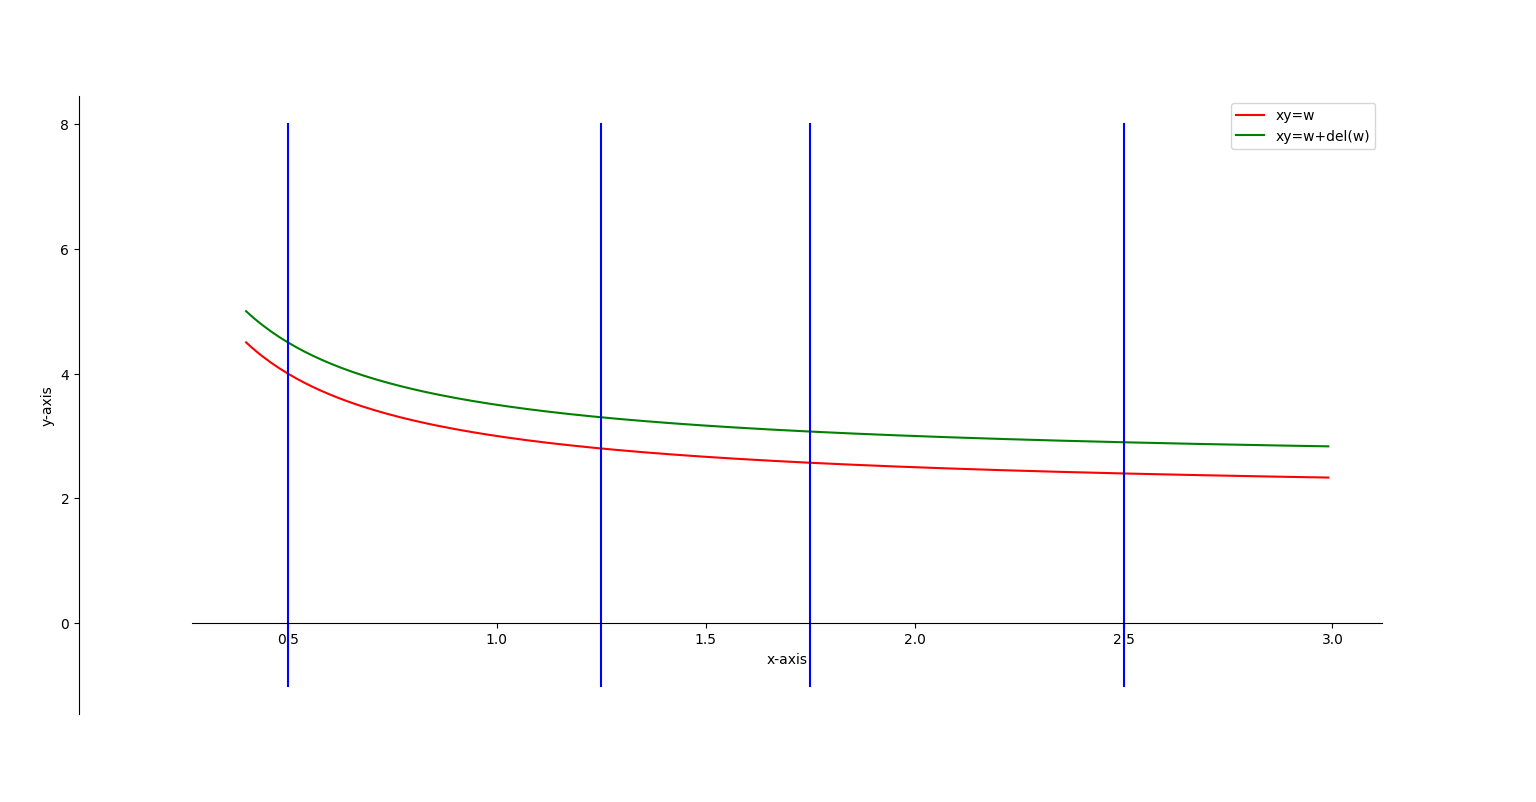
\includegraphics[width=\columnwidth]{figs/assign_8_Figure_2.png}
			\label{Fig2}	
		\end{figure} 
	\end{frame}

  \begin{frame}
	
	\begin{align}
		P\cbrak{x=x_n ,\frac{w}{x_n}\le \underline{y} \leq \frac{w+\Delta w}{x_n}} = p_nf_y\brak{\frac{w}{x_n}}\Delta w   \nonumber
	\end{align} 
	
	\begin{align}
		\implies &\cbrak{w \le \underline{w} \leq w+\Delta w} = \sum_{n} \cbrak{x=x_n ,\frac{w}{x_n}\le \underline{y} \leq \frac{w+\Delta w}{x_n}}   \\
		\implies &f_w\brak{w} \Delta w = \sum_{n} p_nf_y\brak{\frac{w}{x_n}}\Delta z
	\end{align} 
	
  \end{frame}
	
	
\end{document}